\documentclass[12pt]{amsart}
\usepackage{amsaddr}
\usepackage{marktext} 
%% Remove draft for real article, put twocolumn for two columns
\usepackage{svmacro}
\usepackage[utf8]{inputenc}
\usepackage{lineno}
\usepackage[style=alphabetic, backend=biber]{biblatex}
\addbibresource{bibliography.bib}

%% commentary bubble
\newcommand{\SV}[2][]{\sidenote[colback=green!10]{\textbf{SV\xspace #1:} #2}}

%% Title 
\title{ MATH 102: Ideas  of Math }
\author{ Worksheet 10 }

\date{Oct 29, 2024}


\begin{document}

\maketitle

\begin{definition}[Open sentence]
	Open sentence, which are sentences or mathematical
	expressions which
	\begin{enumerate}
		\item do not have a truth value,
		\item depend on some unknown, like a variable $x$ or an arbitrary function $f$ , and
		\item when the unknown is specified, then the open sentence becomes a statement (and so has a truth value).
		      Their truth value depends on which value of $x$ or $f$ one chooses.
	\end{enumerate}
\end{definition}


\begin{definition}[Principle of Explosion]
	From a contradiction, one can derive anything.
\end{definition}

\begin{figure}[ht]
	\begin{center}
		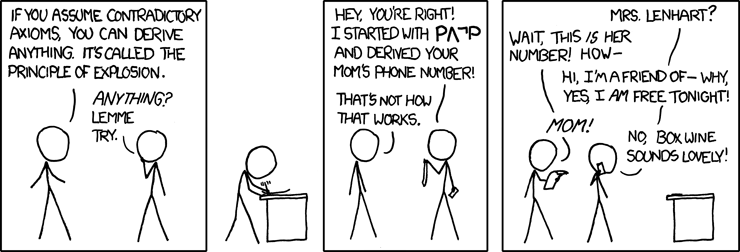
\includegraphics[width=0.7\textwidth]{explo.png}
	\end{center}
\end{figure}


\begin{problem}
From the above principle, write the truth table for $P \implies Q$.
\end{problem}
\vspace{5cm}

\begin{definition}
	The \emph{converse} of $P \implies Q$ is
	$$Q \implies P \,. $$
\end{definition}

\begin{problem}
If $P \implies Q$ is true, is it true $Q \implies P$?
\end{problem}

\vspace{5cm}





\begin{definition}
	Two statements are said to be \emph{logically equivalent} if
	they have the same truth values.

	We denote it by
	\begin{equation*}
		P \iff Q \,.
	\end{equation*}
\end{definition}

\begin{problem}
Relate equivalence symbol ``$\iff$'' and implication symbol ``$\implies$''.
\end{problem}
\vspace{5cm}






\begin{problem}
De Morgan's law for logical statements.
Let $P$ and $Q$ be statements.
Use the truth table to show that for any statement $P$ and $Q$:

\begin{equation*}
	\sim (P \wedge Q ) \iff \sim P \; \vee \sim Q
\end{equation*}

and

\begin{equation*}
	\sim (P \vee Q) \iff \sim P \; \wedge \sim Q
\end{equation*}
\end{problem}

\vspace{5cm}

\begin{problem}
Show that $P \implies Q$ is equivalent to
$\sim P \; \vee Q$.
\end{problem}

\vspace{5cm}


\begin{problem}
Tommy was telling you what he ate yesterday afternoon. He tells you, “I had either popcorn or raisins. Also, if I had cucumber sandwiches, then I had soda. But I didn't drink soda or tea.” Of course you know that Tommy is the world's worst liar, and everything he says is false. What did Tommy eat?

Justify your answer by writing all of Tommy's statements using sentence variables $ P,Q,R,S,T$
, taking their negations, and using these to deduce what Tommy actually ate.
\end{problem}

\newpage

\begin{problem}
You meet two inhabitants $A$ and $B$ on an island.
$A$ says, “Exactly one of us is lying.”
and $B$ says “At least one of us is telling the truth.”.
Who, (if anyone) is telling the truth?
\end{problem}

\end{document}
